\documentclass[border=10pt]{standalone}

\usepackage{tikz}
\usepackage{tikzsymbols}
\usetikzlibrary{calc,patterns,shapes.geometric}

\def\centerarc[#1](#2)(#3:#4:#5){\draw[#1] ($(#2)+({#5*cos(#3)},{#5*sin(#3)})$) arc (#3:#4:#5);}

\begin{document}
	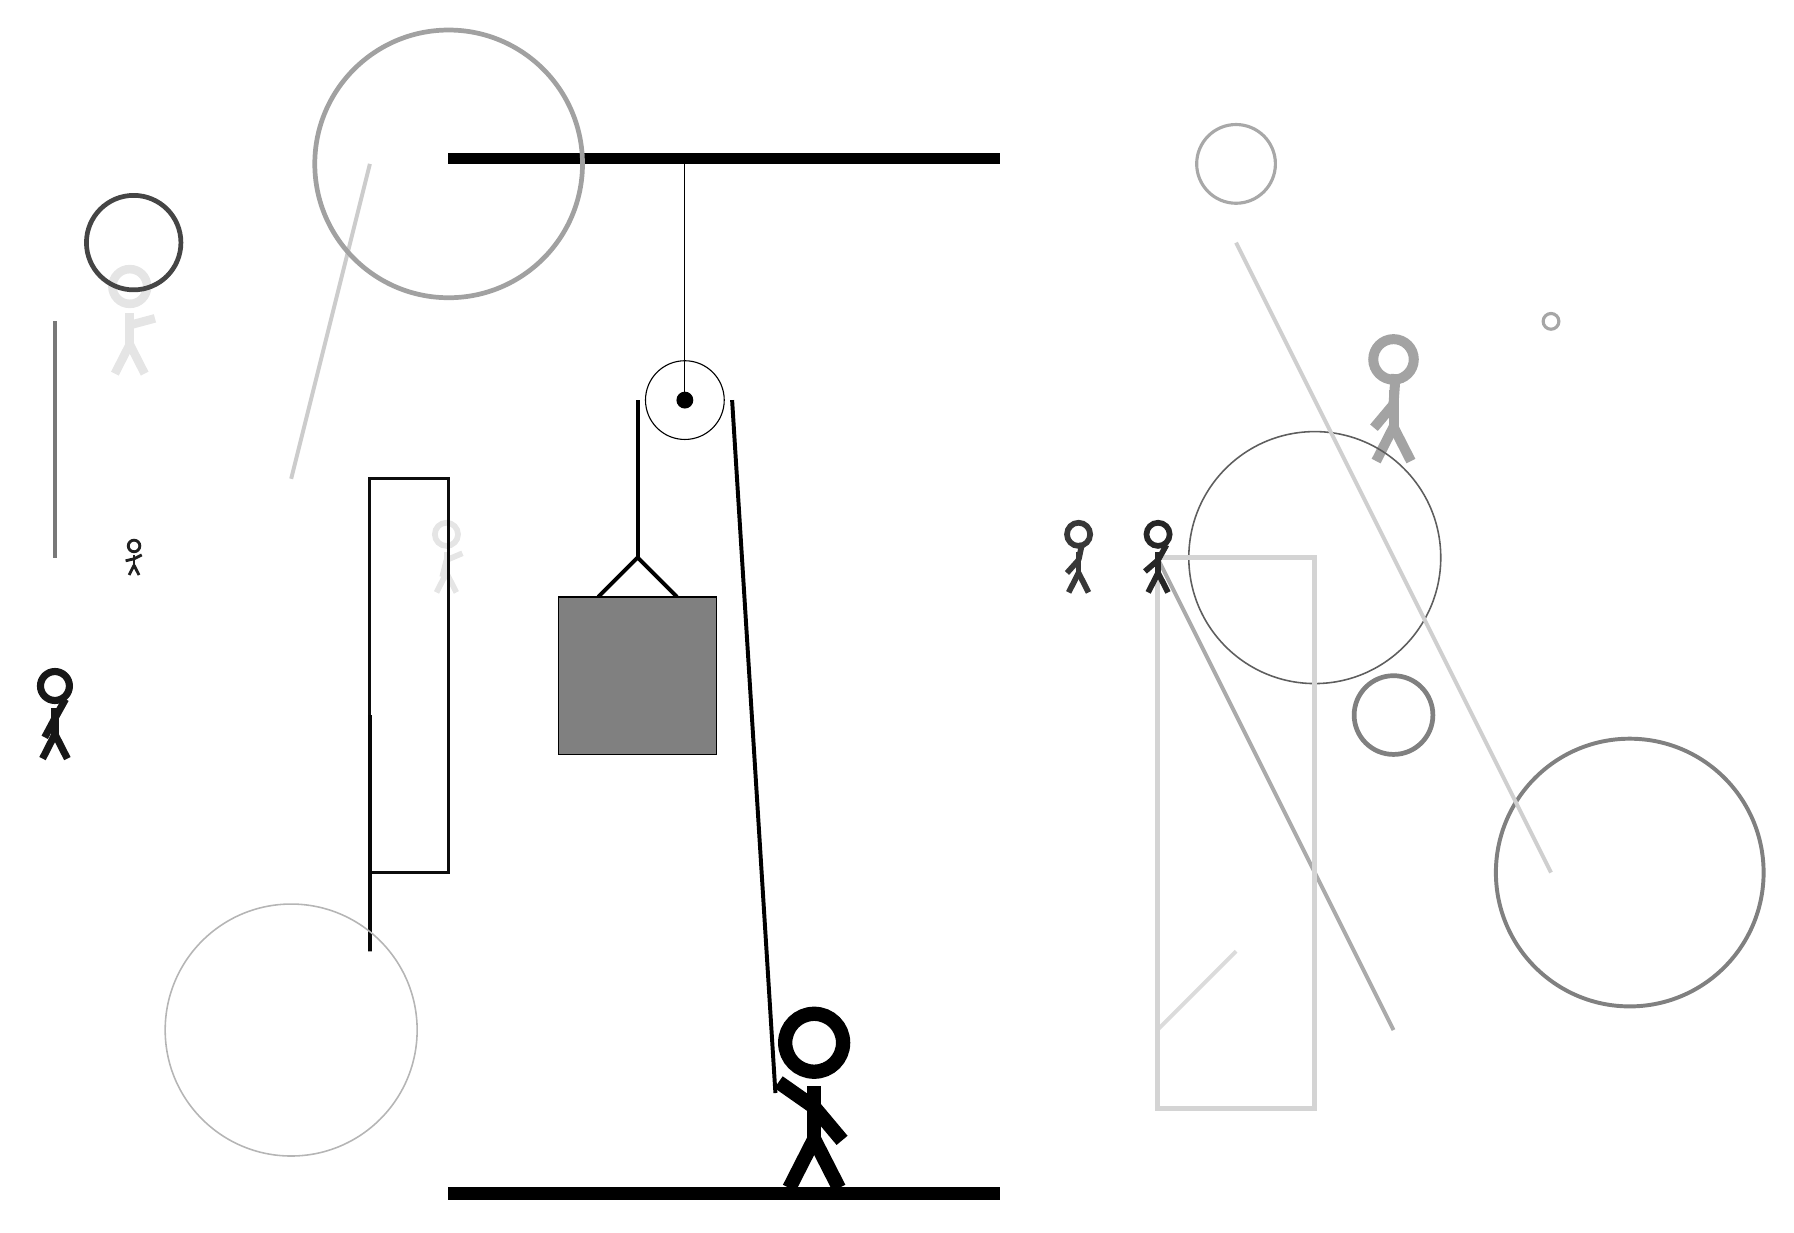
\begin{tikzpicture}
		%%%%% START %%%%%
		
		\draw[fill=black] (-2, 10) rectangle (5, 10.125);
		
		\draw (1, 7) circle (0.5);
		\draw[fill=black] (1, 7) circle (0.1);
		\draw (1, 10) -- (1, 7);
		
		\draw[line width=0.5mm, color=black!14](7, -1) -- (8, 0);
		
		\node[line width=0.6mm, color=black!10] at (-6, 8) {\Strichmaxerl[6][90][15]};
		\node[line width=0.6mm, color=black!10] at (-2, 5) {\Strichmaxerl[4][76][23]};
		\draw[line width=0.4mm, color=black!95] (-2, 1) rectangle (-3, 6);
		
		\node[line width=0.4mm, color=black!36] at (10, 7) {\Strichmaxerl[7][50][86]};
		\node[line width=0.4mm, color=black!78] at (6, 5) {\Strichmaxerl[4][48][78]};
		
		\draw [line width=0.2mm, color=black!63](9, 5) circle (1.6);
		
		\draw[line width=0.5mm, color=black!97] (-3, 0) rectangle (-3, 3);
		\draw[line width=0.5mm, color=black!33](10, -1) -- (7, 5);
		\node[line width=0.7mm, color=black!91] at (-7, 3) {\Strichmaxerl[5][62][61]};
		
		\draw[line width=0.5mm, color=black!20](-3, 10) -- (-4, 6);
		\draw[line width=0.6mm, color=black!17] (7, 5) rectangle (9, -2);
		\node[line width=0.3mm, color=black!87] at (-6, 5) {\Strichmaxerl[2][13][27]};
		
		\draw [line width=0.5mm, color=black!50](13, 1) circle (1.7);
		\draw [line width=0.2mm, color=black!29](-4, -1) circle (1.6);
		\draw [line width=0.4mm, color=black!35](12, 8) circle (0.1);
		\draw[line width=0.5mm, color=black!19](8, 9) -- (12, 1);
		\draw [line width=0.6mm, color=black!50](10, 3) circle (0.5);
		\draw[line width=0.5mm, color=black!53](-7, 8) -- (-7, 5);
		
		\draw [line width=0.6mm, color=black!73](-6, 9) circle (0.6);
		\node[line width=0.5mm, color=black!85] at (7, 5) {\Strichmaxerl[4][41][61]};
		
		\draw [line width=0.6mm, color=black!37](-2, 10) circle (1.7);
		\draw [line width=0.4mm, color=black!34](8, 10) circle (0.5);
		
		\draw[line width=0.5mm] (-0.1, 4.5) -- (0.4, 5.0) -- (0.9, 4.5);
		\draw[fill=black!50] (-0.6, 4.5) rectangle (1.4, 2.5);
		
		\draw[line width=0.5mm] (0.4, 7) -- (0.4, 5.0);
		\centerarc[line width=0.5mm](1, 7)(0:180:0.6);
		\draw[line width=0.5mm](1.6, 7) -- (2.15, -1.8);
		
		\node at (2.6, -1.9) {\Strichmaxerl[10][-35][-50]};
		
		\draw[fill=black] (-2, -3) rectangle (5, -3.15);
		
		%%%%% END %%%%%
	\end{tikzpicture}
\end{document}